% 文中引用说明

\chapter{相关技术理论}

\section{神经网络技术}

\subsection{循环神经网络}

\subsection{长短期记忆}

\section{GAN生成模型选取使用}
\subsection{基础GAN模型的缺陷}
GANs模型的缺点对应着优点,比较明显。由于GANs模型自由度太高,在面对过于清晰的图片等训练样本时,收敛性表现较差,生成模型可能出现退化,重复生成相同样本点,导致判别器无法工作,进而导致模型崩溃。因此,在训练过程中,调整好两个模型网络的平衡与同步非常重要。

正因为GAN模型有着这诸多的缺点,所以要选取比较合适的GAN模型来生成图片。

\begin{figure}[b]
    \centering
    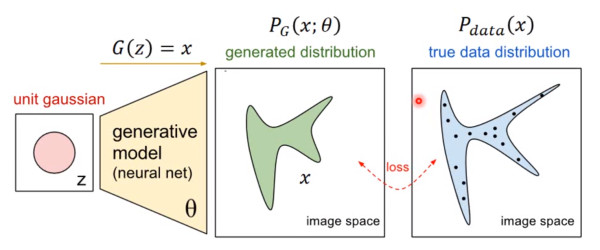
\includegraphics[width=0.8\textwidth]
    {figures/ganprograss.jpeg}\\
    \caption{一般GAN网络模型结构}
    \label{fig:GAN}
  \end{figure}

\subsection{衍生模型分类与特点}
目前对抗生成网络的衍生模型众多,其优化方式大抵由两个大方向衍生而来。一个方向是由损失函数的改变来优化GAN模型的效果,另一个方向则是从模型使用的角度来优化GAN模型的效果。在表~\ref{tab:1.1}中,列举了一些最为常见的GAN模型衍生模型。

\begin{table}[!htb]
    \centering
    \caption{}
    \label{tab:1.1}
    \begin{tabular}{cccc}
        \toprule
        从损失函数角度&\multicolumn{3}{c}{从模型应用角度提出的优化GAN模型}\\
        \cline{2-4}
        提出的优化GAN模型\upcite{fgans}&网络构架角度\upcite{mirza2014conditional}&编码器角度&其他角度改进\\
        \hline
        \multirow{5}{0.3\textwidth}{Least Square GANs, Loss-Sensitive GAN, Fisher GAN, WGAN, WGAN-GP, WGAN-LP, f-GANs\upcite, DRAGAN等}&\multirow{5}{0.19\textwidth}{CGAN, DCGAN, InfoGAN, StackGAN\upcite{zhang2017stackgan}, AL-GAN等}&\multirow{5}{0.19\textwidth}{BEGAN, VAE-GAN, tDCGAN, BiGAN,文献中的算法\upcite{编码器GAN1, 编码器GAN3, 编码器GAN2}等}&\multirow{5}{0.19\textwidth}{LAPGAN, ESRGAN, SRGAN, 3D-GAN, MGAN等}\\ \\ \\ \\ \\
        \bottomrule
    \end{tabular}
\end{table}

图像生成的模型与基于网络构架优化的GAN网络模型最为贴合,本文设计使用StackGAN作为基础,并针对相关实现进行优化。

\subsection{StackGAN及其衍生模型}
Han Zhang et al.在2017年提出了StackGAN模型,创新性地提出了基于栈的对抗式生成网络模型从文本生成图片的方法。

StackGAN和CGAN同属于优化了GAN网络的构架结构的一类GAN模型的分支。其中,StackGAN是对相对朴素的CGAN模型的优化。

\subsubsection{从CGAN到StackGAN}
条件对抗生成网络CGAN
\begin{figure}[t]
    \centering
    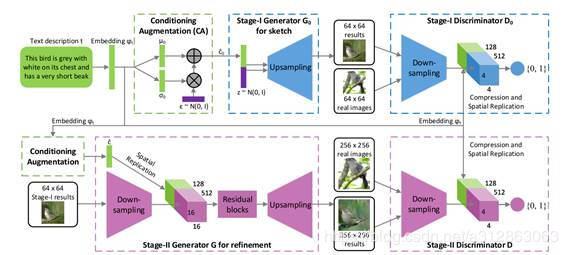
\includegraphics[width=0.8\textwidth]
    {figures/StackGAN.jpg}\\
    \caption{StackGAN构架示意}
    \label{fig:StackGAN}
  \end{figure}
  
在CGAN中,我们将文本作为条件输入生成器和
\subsubsection{StackGAN模型的优势}

\subsubsection{对StackGAN的进一步优化与运用}
同一课题组紧接着提出了StackGAN++\upcite{zhang2018stackgan++},对原有算法进一步进行了优化。

李飞飞课题组的Johnson\upcite{Johnson_2018}在StackGAN模型之上,提出了自己的优化。